\setAuthor{Tundmatu autor}
\setRound{lahtine}
\setYear{2009}
\setNumber{G 8}
\setDifficulty{6}
\setTopic{Geomeetriline optika}

\prob{Kapillaartoru}
Klaasist kapillaartoru on sisemise raadiusega $r$ ja välimise raadiusega $R$. Millist tingimust peavad rahuldama $r$, $R$ ja klaasi murdumisnäitaja $n$, et küljelt vaadates paistaks, et kapillaartoru seinapaksus on null?

\hint
Selleks, et kapillaarisein paistaks null-paksusega, peab kapillaarile puutujana langenud kiir napilt puudutama sisemist õõnsust. Sellisel juhul ei leidu ühtegi kiirt, mis läbiksid kapillaari seina ilma sisemise õõnsuse piirpinnale langemata.

\solu
\begin{center}
	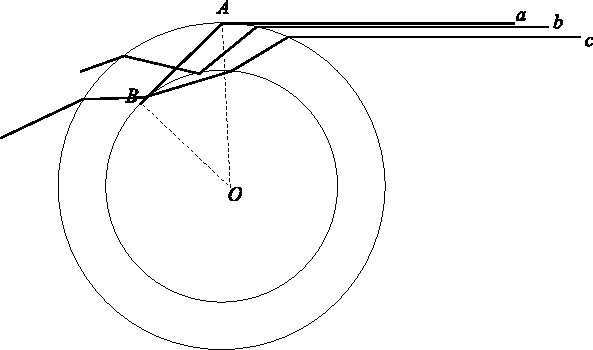
\includegraphics[width=\linewidth]{2009-lahg-08-lah}
\end{center}

Et kapillaarisein paistaks null-paksusega, peab kapillaarile puutujana (punktis$A$, vt joonist) langenud kiir $a$ puudutama sisemist õõnsust (punktis $B$). Sellisel juhul pole ühtegi kiirt, mis läbiks kapillaari seina ilma sisemise õõnsuse piirpinnale langemata (ning vaid kiir $a$ teeb seda puutujana). Kolmnurk $AOB$ on täisnurkne, seetõttu saame murdumisseadusest $n= R/r$. 

Ülesande olukorda edasi analüüsides paneme tähele, et ka võrratuse $r> R/n$ korral puuduvad kiired, mis langevad kapillaari välispinnale, kuid ei lange sisemise õõnsuse piirpinnale; seega ka nende puhul näib kapillaari sein puuduvat. 

Veel paneme tähele, et igal juhul on siiski oluline erinevus ime-õhukese seinaga kapillaarist: kapillaari servale lähedaste kiirte puhul toimub täielik sisepeegeldus sisemise õõnsuse piirpinnalt (joonisel kiir $b$). Visuaalselt paistab see peegel-kihina ja on selgelt eristatav, kui nt kapillaar täita värvilise gaasiga. Samas, see sisepeegeldus kaob, kui kapillaar täita värvilise vedelikuga, mille murdumisnäitaja on $n$.
\probend